\documentclass[twocolumn]{aastex62}
\emergencystretch=1.em

\usepackage{amsmath,amsthm,amsfonts,amssymb,bm}
% for big dot
\makeatletter
\newcommand*\bigcdot{\mathpalette\bigcdot@{.5}}
\newcommand*\bigcdot@[2]{\mathbin{\vcenter{\hbox{\scalebox{#2}{$\m@th#1\bullet$}}}}}
\newcommand{\argmax}{\mathop{\rm arg~max}\limits}
\newcommand{\argmin}{\mathop{\rm arg~min}\limits}

\usepackage{listings}
\usepackage{physics}
\usepackage{multirow}
\usepackage{color}

%\usepackage{subfigure}
\usepackage{textcomp}
\usepackage{epstopdf}
\usepackage{natbib}
\usepackage{commath}
\hypersetup{breaklinks}
\DeclareMathOperator{\arccosh}{arccosh}
\newcommand \figPath{./}
\newcommand \redColor{\color{red}}
\renewcommand\labelenumi{(\roman{enumi})}
\renewcommand\theenumi\labelenumi

\usepackage{algorithm,algcompatible}

%\DeclareMathOperator*{\argmax}{\arg\!\max}
\algnewcommand\INPUT{\item[\textbf{Input:}]}
\algnewcommand\OUTPUT{\item[\textbf{Output:}]}

\makeatother
%\newcommand{\jcap}{JCAP}

\begin{document}
\title{Sparsity Weak Lensing $3$-D Density Map Reconstruction: 
Reducing the line-of-sight smearing.}
%\author{Xiangchong Li}
%\affiliation{Department of Physics, University of Tokyo, Tokyo 113-0033, Japan}
%\affiliation{Kavli Institute for the Physics and Mathematics of the Universe (WPI),\\
%University of Tokyo, Kashiwa 277-8583, Japan}
%\author{Masamune Oguri}
%\affiliation{Department of Physics, University of Tokyo, Tokyo 113-0033, Japan}
%\affiliation{Kavli Institute for the Physics and Mathematics of the Universe (WPI),\\
%University of Tokyo, Kashiwa 277-8583, Japan}
%\affiliation{Research Center for the Early Universe, University of Tokyo, Tokyo 113-0033, Japan}
%\author{Wentao Luo}
%\affiliation{Kavli Institute for the Physics and Mathematics of the Universe (WPI),\\
%University of Tokyo, Kashiwa 277-8583, Japan}
%\author{HSC Collaboration}
%\noaffiliation
%\email{xiangchong.li@ipmu.jp}

\begin{abstract}
A new method is developed to reconstruct $3$-D density contrast maps from photometric weak lensing shear measurements.
The $3$-D density contrast maps is modeled as a summation of NFW basis atoms which have $2$-D multi-scale NFW surface 
density profiles on the transverse plane and $1$-D Dirac delta functions in the line-of-sight direction. With the prior 
assumption that the density fields can be sparsely represented by the NFW basis atoms, it is reconstructed using an 
oracle algorithm: adaptive lasso. Our method is tested with realistic simulations using the HSC-like shape noise and 
photo-$z$ uncertainty.
{\redColor{Add descriptions on the outcomes of the test on the simulations.}}
\end{abstract}

\section{Introduction}

\begin{figure*}[!t]
    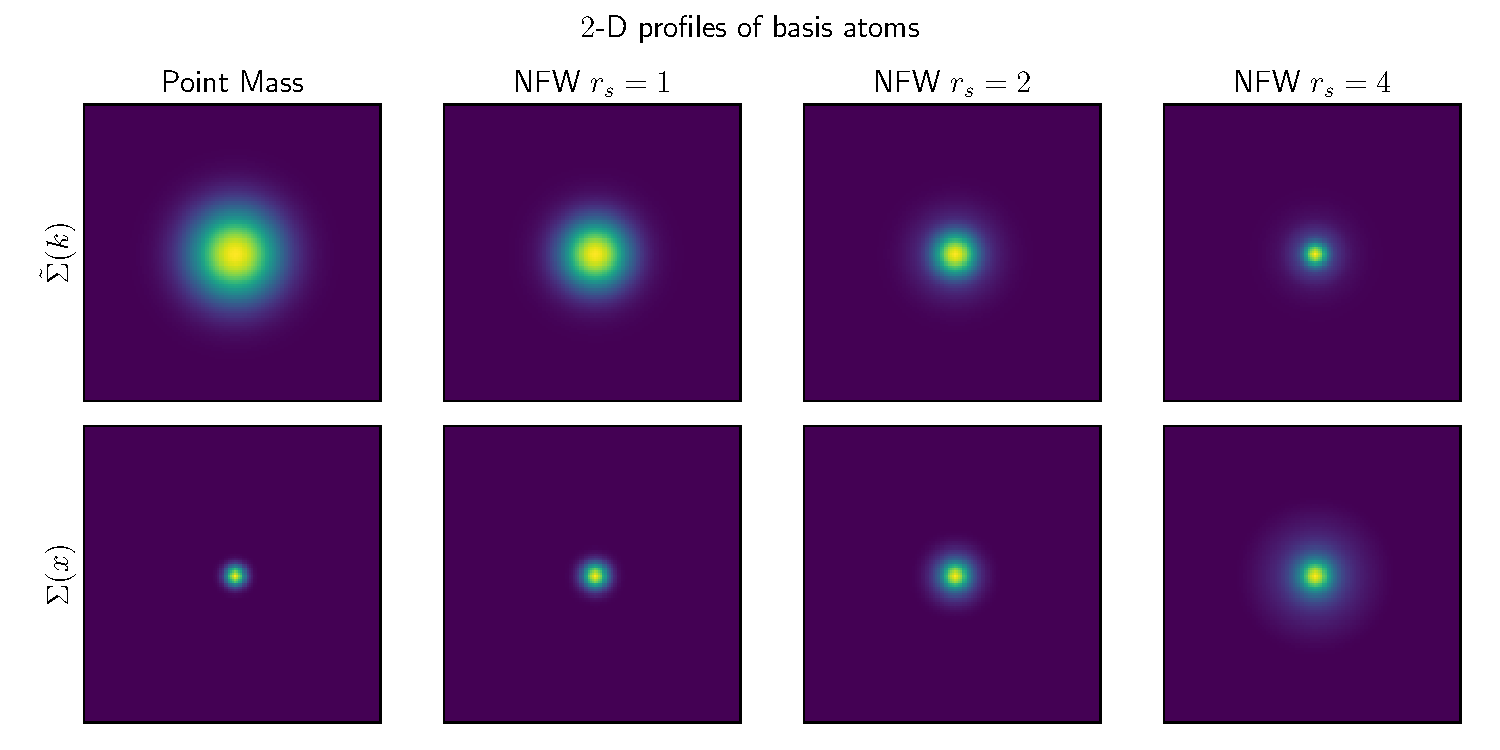
\includegraphics[width=1.\textwidth]{nfwlet-atom-2D.pdf}
    \caption{The smoothed basis atoms. The first row shows the smoothed basis atoms in Fourier space 
            and the second row shows the smoothed basis atoms in Real space. 
            The first column is point mass atom and the other columns are multi-scale NFW atoms.
            The smoothing kernel is Gaussian with scale of $1.5$ pixels.} \label{fig-atoms2D}
\end{figure*}

\begin{figure}
 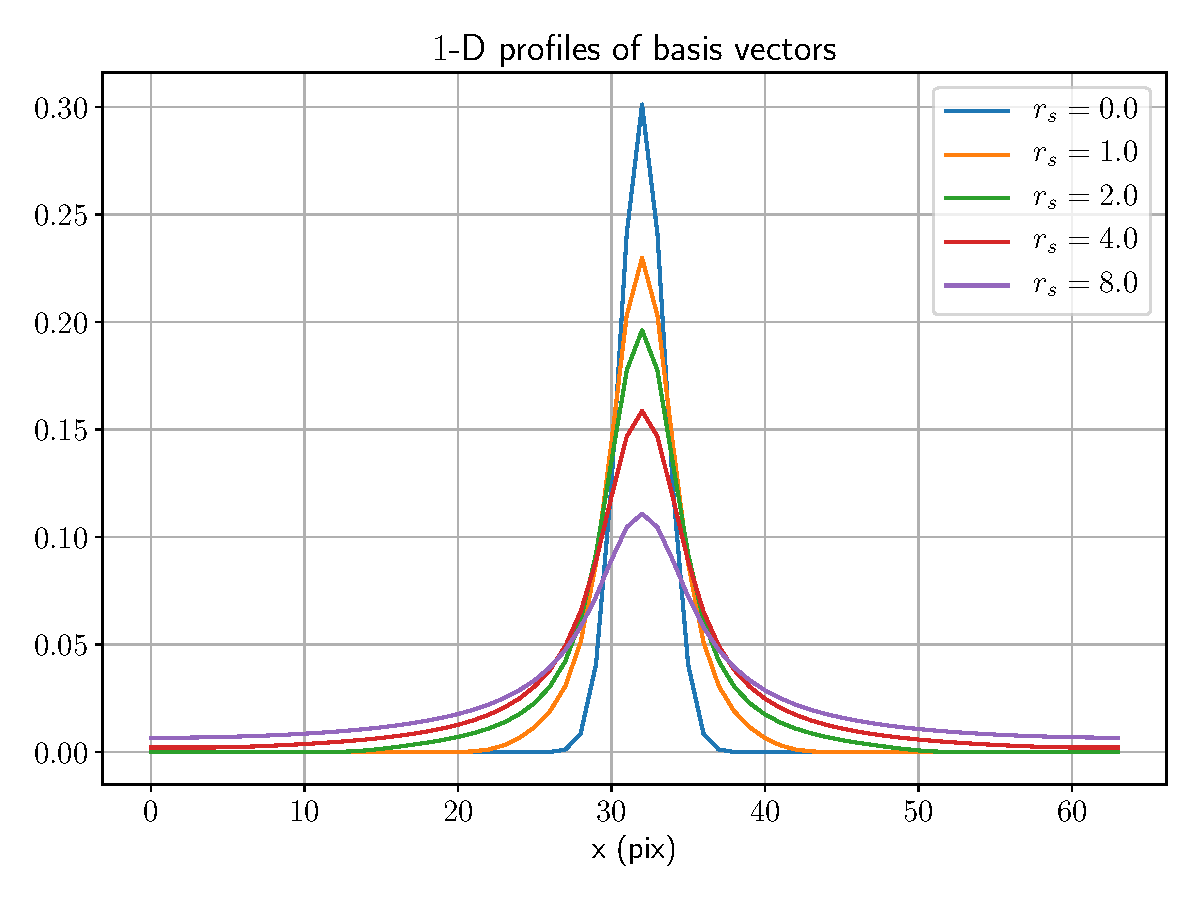
\includegraphics[width=0.5\textwidth]{nfwlet-atom-1D.pdf}
 \caption{The $1$-D slices for smoothed basis atoms at $x=0$. The corresponding $2$-D profiles are shown in Figure 
        \ref{fig-atoms2D}.} \label{fig-atoms1D}
\end{figure}

Light from distant galaxies is distorted by the intervening inhomogeneous density distribution along the line-of-sight
due to the influence of gravity. As a result of the light distortion, the shapes of the background galaxies are coherently
sheared. Such effect, which is known as weak lensing, imprints the information of foreground mass density distribution
to the background galaxy images and offers a direct probe into the mass density distribution in our universe
\citep[see][for recent reviews]{revKilbinger15,revRachel17}.

The expected shear measurements ($\gamma$) on distant galaxies are related to the 
foreground density contrast field ($\delta$) through a linear transformation
\begin{equation} \label{eq-intro-delta2shear}
 \gamma=\mathbf{T} \delta,
\end{equation}
where $\mathbf{T}$ is used to denote the linear transformation operator which includes not only physical lensing effect
but also systematic effects from observations (e.g. pixelization and smoothing of shear field in
transverse plane, photo-$z$ uncertainty).

Several large scale surveys target to study the weak lensing effect at high precision level (e.g. HSC \citep{HSC1-data}, KIDS
\citep{KIDS13}, DES \citep{DES05}, LSST \citep{LSSTScienceBook}, Euclid \citep{Euclid2011}, WFIRST \citep{WFIRST15}).

The primary goal of most weak lensing surveys is to constrain the cosmology model through $2$-point correlations. The studies
include galaxy-galaxy lensing which cross correlating the shear field ($\gamma$) with the positions of foreground galaxies
\citep{gglens-GAMA-Han2014,gglens-BossCFHTMore2015,gglens-DES1},
and cosmic shear which auto-correlates the shear measurements
\citep{cosmicShearRealKids450,cosmicShear-DES1,cosmicShear_HSC1_Chiaki2019,cosmicShear_HSC1_Hamana2019}.
Since shear is directly related to the matter distribution as shown in eq. (\ref{eq-intro-delta2shear}), Galaxy-galaxy lensing
probes into the correlation between the matter field and galaxy field, on the other hand, cosmic shear probes into the
auto-correlation of matter field.

Reconstructions of density map from shear measurements also receive considerable interest. $2$-D density map reconstruction 
which recover an integration of projected mass along the line-of-sight has been well studied within the community
\citep{massMap-KS1993,WL-massMap-Glimpse2D-Lanusse2016,sparseBaysianMassMap-Price2020}
and applied to large scale surveys \citep{HSC1-massMaps,massMapDES-Chang2018,DES-SV-massMap-sparsity}. However, the 
reconstruction of $3$-D mass map is still a challenging task.

In order to fully reconstruct the $3$-D mass density distribution ($\delta$) from the photometric shear observations ($\gamma$),
the density contrast field is modeled as a summation of basis atoms in a model dictionary
\begin{equation} \label{eq-intro-dict}
 \delta= \mathbf{\Phi} x,
\end{equation}
where $\mathbf{\Phi}$ is the transformation operator from the parameters in the dictionary space to the density contrast 
and $x$ denotes the parameters. \citet{LSS-massMap-Wiener-Simon2009} reconstruct the density field
in Fourier space, which is equivalent to model the mass field with sinusoidial functions. On the other hand,
\citet{LSS-massMap-Glimpse3D-Leonard2014} models the mass field with Starlets \citep{Starlet-Starck2015}.

The projection coefficients are estimated through optimizing a loss function with regularization. The estimator is
generally defined as
\begin{equation}
\hat{x}=\argmin_{x} \left\{ \frac{1}{2}\norm{\Sigma^{-\frac{1}{2}}(\gamma- \mathbf{T\Phi} x)}_2^2+ \lambda C(x) \right\},
\end{equation}
where $\norm{\Sigma^{-\frac{1}{2}}(\gamma - \mathbf{T\Phi} x)}_2^2$ is the chi-square term\footnote{weighted by the
inverse of the diagonal covariance matrix of error on the shear measurements ($\Sigma$).} measuring
the residuals between the prediction and the data, while $C(x)$ is the regularization term measuring the deviation of
the estimation of the parameter ($x$) from the prior assumptions. Such estimation prefers the parameters that are able
to describe the observations and also align with the prior assumptions. The regularization parameter $\lambda$ adjusts 
the relative weight between the observations and prior assumptions in the optimization process.

\citet{LSS-massMap-Wiener-Simon2009} propose to use the Wiener filter, which is also known as $l^2$ ridge regulation 
($C=\norm{x}^2_2$), to find a solution in Fourier space. \citet{HSC1-massMaps} apply the method of 
\citet{LSS-massMap-Wiener-Simon2009} to the first year data of the Hyper Suprime-Cam Survey \citep{HSC1-data}. 
However, the density maps reconstructed by this method suffer from a smearing along the line-of-sight direction with 
a standard deviation of $\sigma_z=0.2 \sim 0.3$.

\citet{LSS-massMap-Glimpse3D-Leonard2014} propose to use a derivative version of $l^1$ lasso regulation ($C=\norm{x}^1_1$) 
to find a sparse solution in the Starlets dictionary space \citep{Starlet-Starck2015}. \citet{LSS-massMap-Glimpse3D-Leonard2014}
apply a greedy coordinate descent algorithm, which selects the steepest coordinate in each iteration, to find the minima 
of a non-convex loss function penalized with the firm thresholding function. \citet{LSS-massMap-Glimpse3D-Leonard2014} 
significantly reduce the smearing along the line-of-sight, however, the stability of the non-convex optimization and
greedy coordinate descent algorithm has not been fully justified. Moreover, the Starlets functions are not designed to 
model the profile of clumpy mass in the universe. 

$N$-body simulations have shown that the dark matter is distributed in halos connected by filaments, and the density 
profile of a single halo follows the NFW function \citep{halo-NFW1997ApJ}.
We construct a dictionary with multi-scale NFW atoms.  The atoms follow multi-scale surface density profiles of NFW 
functions \citep{haloModel-TJ2003-3pt} on the transverse plane. We follow \citet{LSS-massMap-Glimpse3D-Leonard2014} 
to neglect the depth of halos since the resolution scale of the reconstruction in the line-of-sight direction is much 
larger than the scales of halos. Therefore, we set the profile of the NFW atoms in the line-of-sight as the Dirac delta 
function. The multi-scale NFW atoms are used to model the profiles of halos which is assumed to be sparsely distributed 
in the universe. With the sparsity prior, the adaptive lasso regularization \citep{AdaLASSO-Zou2006} is used to reconstruct 
the density field. We find that, in contrast to the standard lasso estimator which smears the structure along the line-of-sight,
the addaptive lasso is able to significantly reduce the smearing effect.

Comparing with \citet{LSS-massMap-Glimpse3D-Leonard2014}, our dictionary is built up to describe the clumpy mass 
in the universe which has a clear physical motivation. Furthermore, the adaptive lasso algorithm is strictly convex and 
can be directly optimized with the FISTA algorithm \citep{FISTA-Beck2009} without relying on any greedy coordinate 
descent approaches.  The stability of this convex optimization has been well studied.

This paper is organized as follows.
Section \ref{sec:Method} proposes the new method for $3$-D density map reconstruction.
Section \ref{sec:Test} Tests our algorithm on HSC-like simulations.
Section \ref{sec:Sum} summarizes and discusses the future development of the method.

\section{Methodology}
\label{sec:Method}

\begin{figure}[!t]
 \centering
 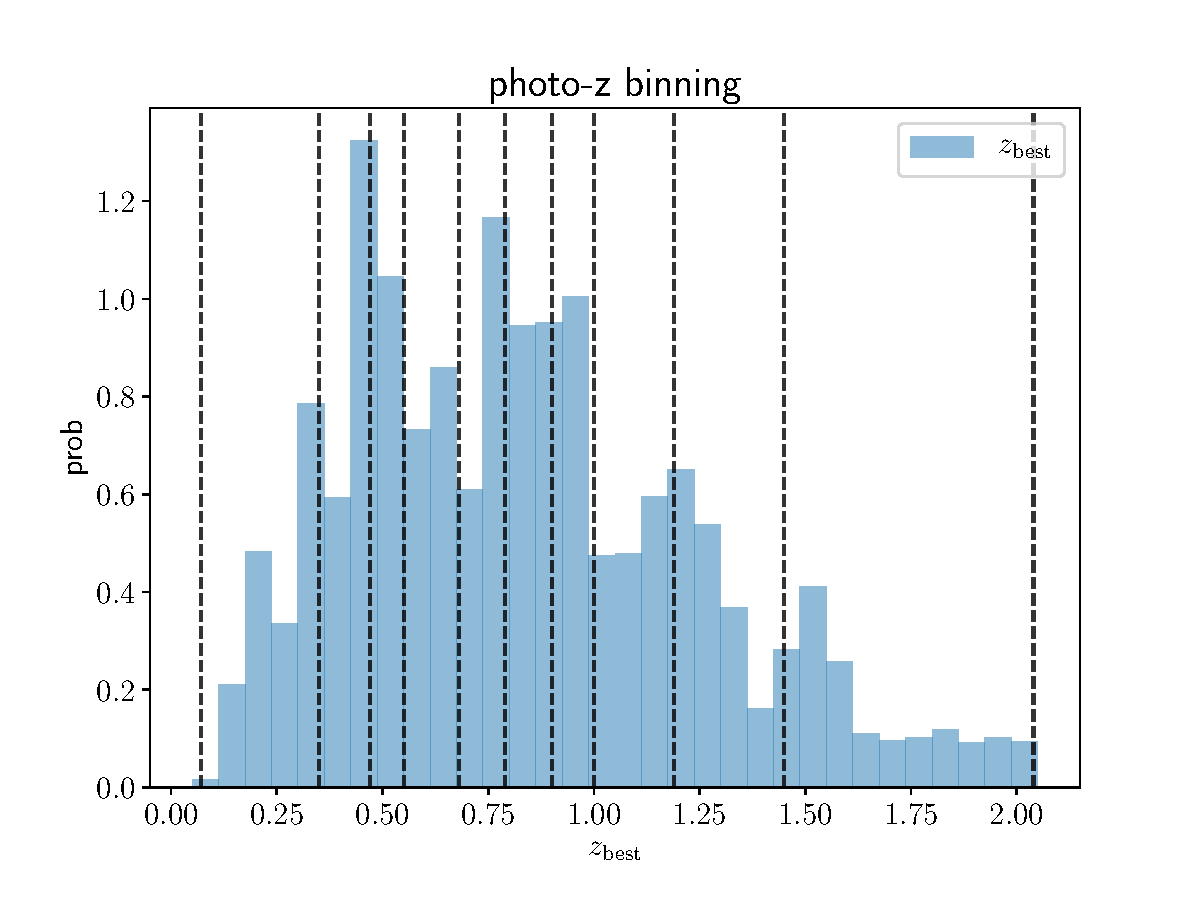
\includegraphics[width=0.5\textwidth]{photo-z_binning.pdf}
 \caption{The source galaxies are binned into $10$ redshift bins according to their MLZ best photo-$z$ estimation.
        The blue histogram is the number distribution of the best photo-$z$ estimation. The vertical dashed lines
        are the bounds of bins. The galaxies are evenly distributed in each bins.} \label{fig-bestpz}
\end{figure}

We first review the lensing process in section \ref{subsec:method-delta2shear}.
Then, we introduce the dictionary used to model the foreground density maps in section \ref{subsec:method-dictionary}.

Subsequently, in section \ref{subsec:method-Systematics}, we discuss several systematic effects from observations which 
include photo-$z$ uncertainty (section \ref{subsec:method-photoz}),
smoothing (section \ref{subsec:method-smoothing}),
masking(section \ref{subsec:method-msknoise}),
and pixelization (section \ref{subsec:method-pixel}).

Finally, we find the sparse solution in section \ref{subsec:method-reconstruction} using the adaptive lasso algorithm 
\citep{AdaLASSO-Zou2006} optimized with the FISTA alogrithm \citep{FISTA-Beck2009}.


\subsection{Lensing}
\label{subsec:method-delta2shear}

\begin{figure}[!t]
 \centering
 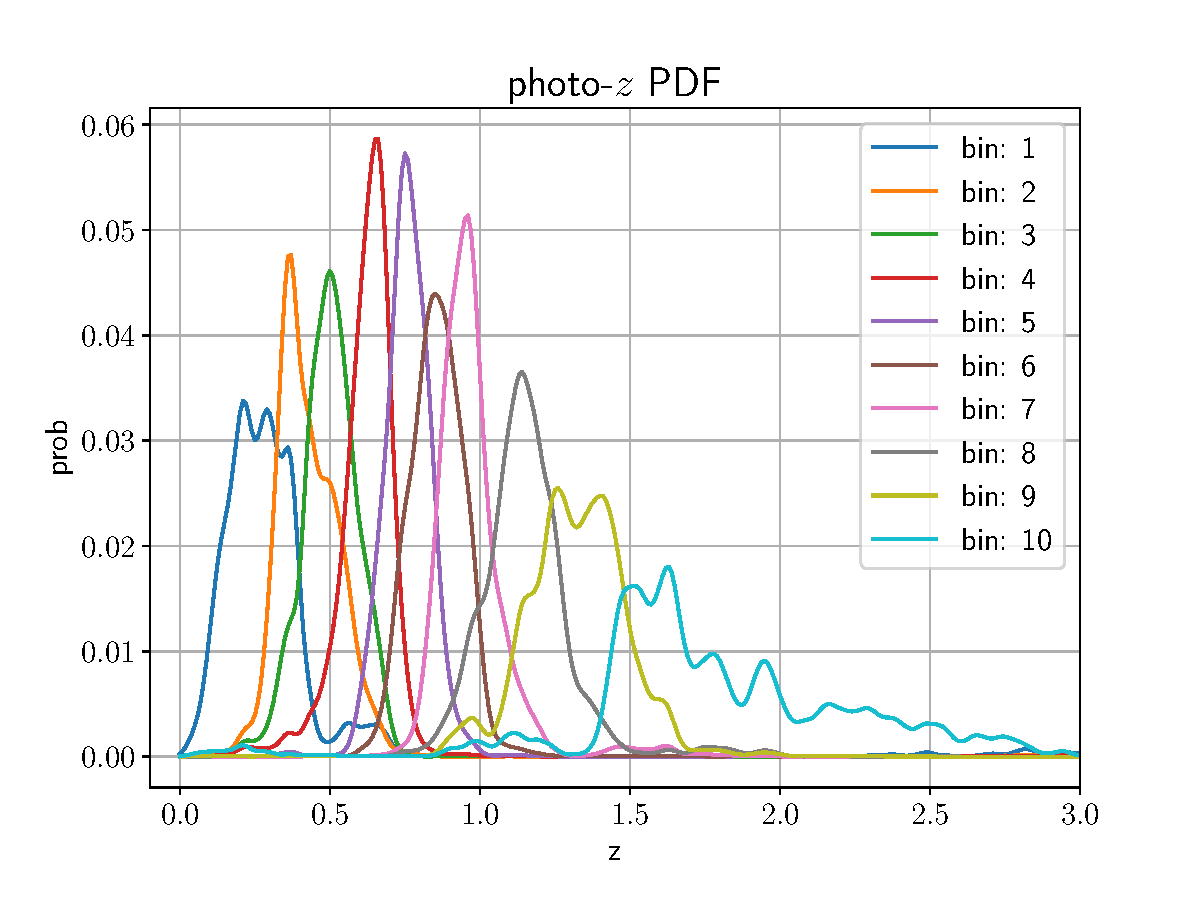
\includegraphics[width=0.5\textwidth]{mlz-poz.pdf}
 \caption{The average PDF of MLZ photo-$z$ error for $10$ source redshift bins.}\label{fig-pdfpz}
\end{figure}

The lensing convergence map at the comoving distance $\chi_s$ caused by the foreground inhomogeneous
density distribution at the comoving distance $\chi_l$ ($\chi_l< \chi_s$) along the line-of-sight is
\begin{equation}
\kappa(\vec{\theta},\chi_s)=\frac{3H_0^2\Omega_M}{2 c^2} \int_0^{\chi_s} d\chi_l \frac{\chi_l \chi_{sl}}{\chi_s}
\frac{\delta(\vec{\theta},\chi_l)}{a(\chi_l)},
\end{equation}
where $\delta=\rho(\vec{\theta},\chi_l)/\bar{\rho}-1$ is the density contrast
at the position of lens, $H_0$ is the Hubble parameter, $\Omega_M$ is the matter density parameter, $c$ is the speed
of light, and $a(\chi_l)$ is the scale parameter at the lens position.

Substitute comoving distance ($\chi$) with redshift ($z$), we have
\begin{equation}\label{eq-delta2kappa}
\kappa(\vec{\theta},z_s)=\int_0^{z_s} dz_l K(z_l,z_s)\delta(\vec{\theta},z_l).
\end{equation}
where $K(z_l,z_s)$ is the lensing kernel defined as
\begin{equation}
K(z_l,z_s) =
\begin{cases}
\frac{3H_0\Omega_M}{2 c} \frac{\chi_l \chi_{sl} (1+z_l)}{\chi_{s} E\left(z_l\right)} & (z_s>z_l),\\
0&(z_s \leq z_l),
\end{cases}
\end{equation}
where $E(z)$ is the Hubble parameter as a function of redshift, in units of $H_0$.

\begin{figure*}[!t]
 \centering
 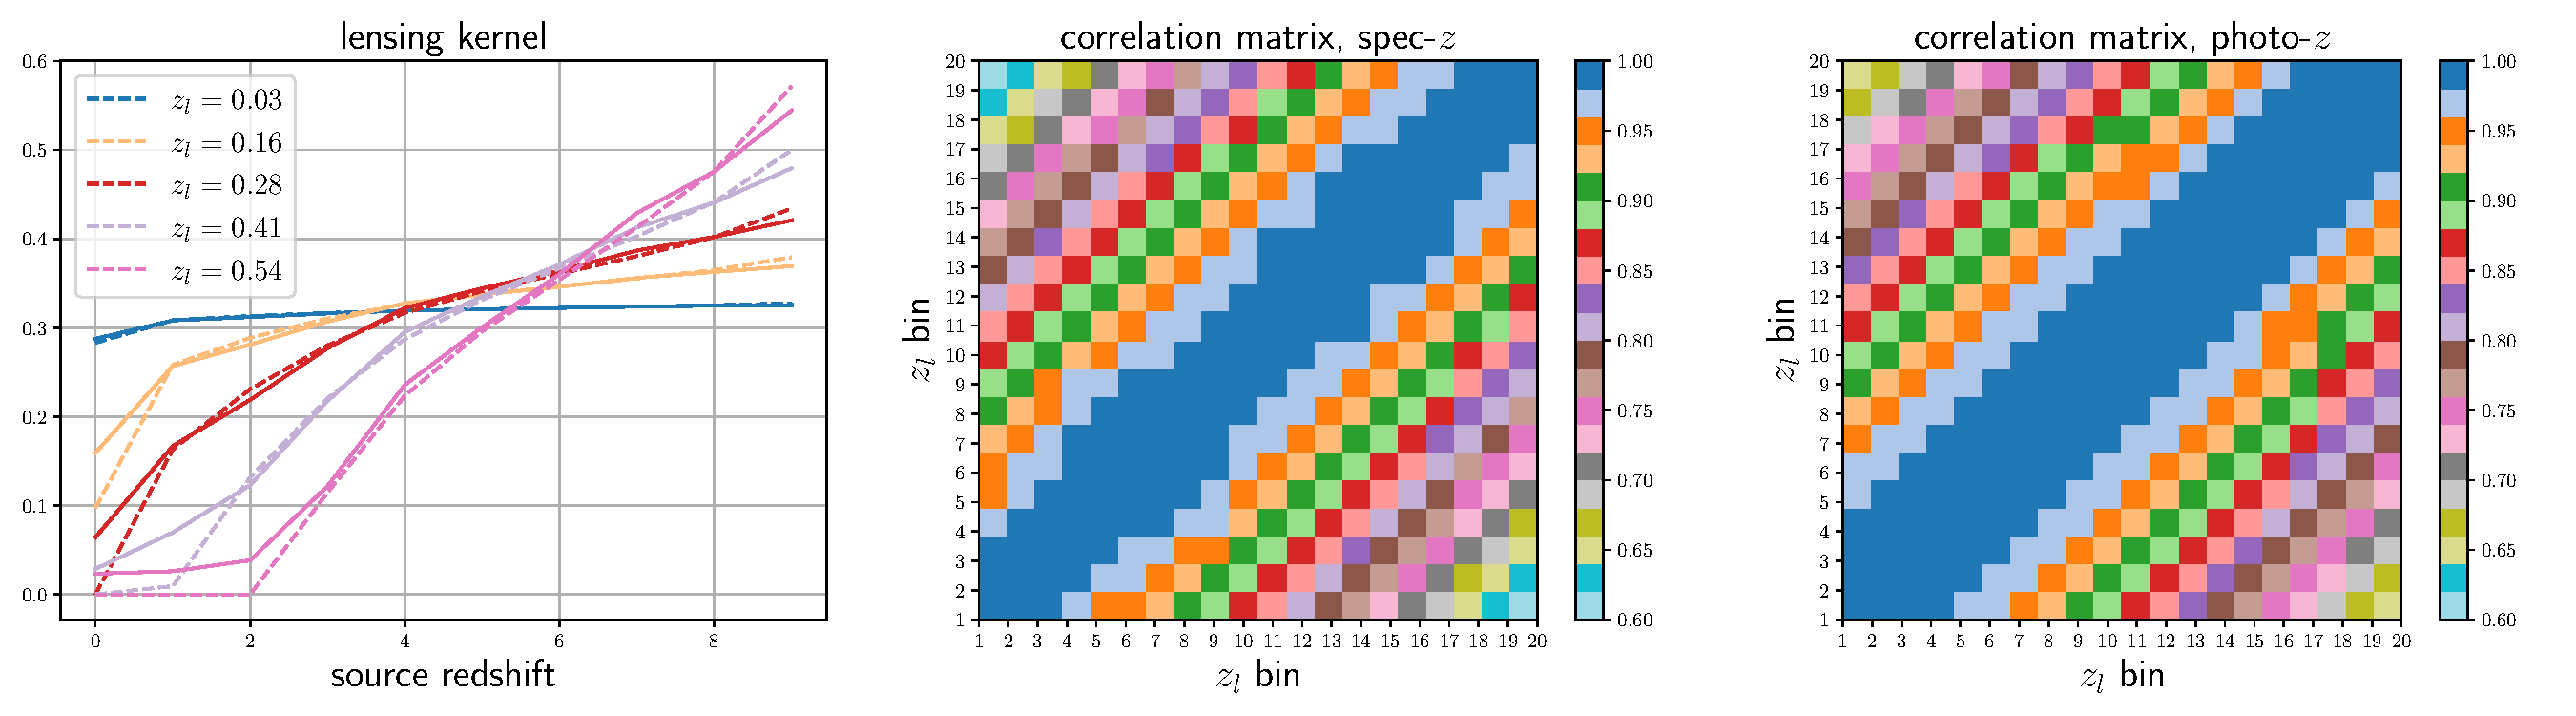
\includegraphics[width=1.\textwidth]{lensing_kernel.pdf}
 \caption{The left panel shows the lensing kernels for five different lens redshifts. The dashed lines are the 
        kernels for spectroscopic redshift which assumes that the redshifts of source galaxies are precisely 
        estimated. The solid lines are for photometric redshifts which accounts for the influence of photometric 
        redshift uncertainty. The other two panels show the correlation between lensing kernels of different 
        lens redshifts. The middle panel is for spectroscopic redshift and the right panel is for photometric 
        redshifts. The lensing kernels are normalized so that the diagonal elements of the correlation matrices
        equal one.}\label{fig-corlensKer}
\end{figure*}

As shown in \citet{massMap-KS1993}, the shear field is related to the kappa field at the same redshift plane
via
\begin{equation}\label{eq-kappa2gamma}
\gamma_L(\vec{\theta},z_s) = \int  d^2 \theta' D(\vec{\theta}-\vec{\theta'}) \kappa(\vec{\theta'},z_s),
\end{equation}
where
\begin{equation}
D(\vec{\theta})=-\frac{1}{\pi}(\theta_1-i\theta_2)^{-2}.
\end{equation}
Here we denote the physical shear distortion field as $\gamma_L$ and we note that the final observed shear measurements 
are also physical shear distortions influenced by systematic errors from observatins. The systematic error will be discussed 
in Section \ref{subsec:method-Systematics}.

Combining equation (\ref{eq-delta2kappa}) with equation (\ref{eq-kappa2gamma}), the expectation of lensing shear signal is 
\begin{equation}\label{eq-delta2gammat}
\gamma_L(\vec{\theta},z_s) = \int_0^{z_s} dz_l K(z_l,z_s) \int d^2 \theta' \vec{D}(\vec{\theta}-\vec{\theta'}) \delta(\vec{\theta'},z_l).
\end{equation}

To simplify the expression, we define the lensing transform operator as
\begin{equation}
\mathbf{Q}=\int_0^{z_s} dz_l K(z_l,z_s) \int d^2 \theta'  \vec{D}(\vec{\theta}-\vec{\theta'}),
\end{equation}
and eq. (\ref{eq-delta2gammat}) is simplified to
\begin{equation} \label{eq-delta2gammat-simp}
\gamma_L=\mathbf{Q}\delta.
\end{equation}

\subsection{Dictionary}
\label{subsec:method-dictionary}

\begin{figure*}[!t]
\centering
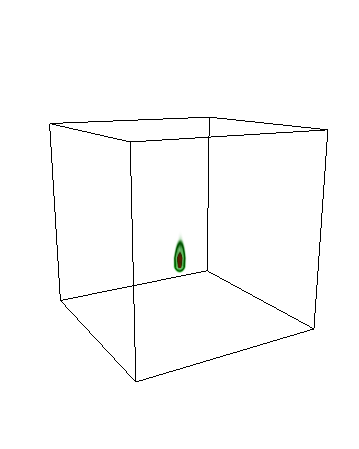
\includegraphics[width=0.42\textwidth]{delta-3-7-pz-nn-lasso.png}
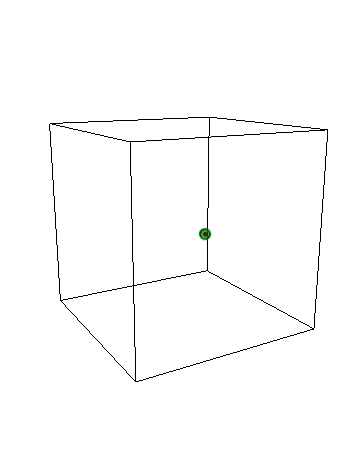
\includegraphics[width=0.42\textwidth]{delta-3-7-pz-nn-alasso.png}
\caption{The result of density map reconstruction with standard lasso (left) and adaptive lasso (right). The input density 
        map is from a NFW halo with mass $M_{200}=10^{15} ~h^{-1}M_{\odot}$ at redshift $0.35$. The lasso reconstruction 
        smear the density field along the line-of-sight direction. Noises on shear measurements are neglected in the 
        simulation.} \label{fig-lassoVsadaLasso}
\end{figure*}

The density contrast field is modeled as a summation of basis atoms in the dictionary 
\begin{equation}\label{eq-x2delta}
\delta(\vec{r}) = \sum_{s=1}^{N} \int d^3 r' \phi_s(\vec{r}-\vec{r'}) x_s(\vec{r'}),
\end{equation}
where $\phi_s(\vec{r})$ are the basis atoms of the dictionary. The basis atoms have `$N$' different scales and the atoms
in each scale frame are shifted by $\vec{r'}$ to form basis at different positions. $x_s(\vec{r'})$ is the projection 
coefficients of the density contrast field onto the basis atoms.

These basis atoms are constructed with multi-scale NFW atoms which are denoted as $\{\phi_1,...,\phi_N\}$.
On the transverse plane, the NFW atoms follow surface density profiles of NFW halos
\citep{haloModel-TJ2003-3pt} with scale radius $\theta_\alpha$ and truncation radius $c \theta_\alpha$ ,
where $c$ is the concentration of NFW halos.
As the scales of halos are much less than the reachable redshift resolution, we neglect the depth of halo on the
line-of-sight direction and set the profiles of NFW atoms in the line-of-sight direction to $1$-D Dirac delta 
functions as suggested by \citep{LSS-massMap-Glimpse3D-Leonard2014}. 
The multi-scale NFW atoms are defined as
\begin{equation}
\begin{split}
\phi_\alpha(\vec{r}) =&\frac{f }{2 \pi \theta_\alpha^2 } F(|\vec{\theta}|/\theta_\alpha) \delta_D(z),\\
&  (s=1..N)
\end{split}
\end{equation}
where
\begin{equation}
F(x)=
\begin{cases}
-\frac{\sqrt{c^2-x^2}}{(1-x^2)(1+c)} + \frac{\arccosh \left(\frac{x^2+c}{x(1+c)}\right)}{(1-x^2)^{3/2}}  & (x<1),\\
\frac{\sqrt{c^2-1}}{3(1+c)} (1+\frac{1}{c+1}) & (x=1),\\
-\frac{\sqrt{c^2-x^2}}{(1-x^2)(1+c)} + \frac{\arccos\left(\frac{x^2+c}{x(1+c)}\right)}{(x^2-1)^{3/2}} & (1<x\leq c),\\
0& (x>c).
\end{cases}
\end{equation}
$f=1/[\ln (1+c)-c/(1+c)]$. In this work, we fix $c=4$ for NFW atoms in different scale frames.

To simplify the notation, we define the projection parameters as a column vector:
$x=\begin{pmatrix}
x_{0}\\
x_{1}\\
...\\
x_{N}
\end{pmatrix}$,
and the dictionary transform operator as a row vector:
\begin{equation}
\mathbf{\Phi}=\begin{pmatrix}
\int d^3r\phi_0(\vec{r}) ~\int d^3r \phi_1(\vec{r})~ ...~\int d^3r \phi_{N}(\vec{r})
\end{pmatrix}.
\end{equation}
We substitute eq. (\ref{eq-x2delta}) into eq.(\ref{eq-delta2gammat})
\begin{equation}\label{eq-x2gammat}
\gamma_L=\mathbf{Q}\mathbf{\Phi} x.
\end{equation}

In this paper dictionary constructed with point mass atoms is used to compare with the dictionary of multi-scale atoms.
The point mass atoms is a $3$-D Dirac function defined as follows
\begin{equation}
\phi_{\rm{PM}}(\vec{r})= \delta_D(\theta_1) \delta_D(\theta_2) \delta_D(z).
\end{equation}

The $2$-D profiles of the point mass atom and the multi-scale NFW atoms on the transverse plane are shown in Figure 
\ref{fig-atoms2D}. The $1$-D slices of the profiles are demonstrated in Fiugre \ref{fig-atoms1D}. Note that these profiles 
are smoothed with a Gaussian kernel and pixelized into evenly spaced grids. The smoothing operator is described in 
Section \ref{subsec:method-smoothing} and the pixelization operator is described in Section \ref{subsec:method-pixel}.

\subsection{Systematics}
\label{subsec:method-Systematics}

The observed shear measurements are deviated from the physical shear prediction due to the systematic 
errors from observations. The influence of systematics is carefully studied and incorporated into the forward 
modeling in this section.

\subsubsection{Photo-$z$ Uncertainty}
\label{subsec:method-photoz}

The photometric redshifts of source galaxies in the current large scale survey are estimated with a limited number of 
board photometric bands (e.g. $9$ bands for KIDS$+$VIKING survey, $5$ bands for DES survey and HSC survey). As a result, 
the estimated redshifts of galaxies suffer from much larger uncertainties, comparing with redshifts estimated with 
spectroscopic observations. Such photo-$z$ uncertainty smears the lensing kernels statistically since a galaxy with a 
best fit photo-$z$ estimation of $z_s$ has possibilities of being actually located at different redshifts ($z$).
The probability function for the photo-$z$ uncertainty is denoted as $P(z|z_s)$ and the expected shear distortion on 
the galaxy is
\begin{equation}\label{eq-delta2gamma-poz}
\gamma_L(\vec{\theta},z_s) \rightarrow \int dz_s P(z|z_s) \gamma_L(\vec{\theta},z_s).
\end{equation}
With the definition of photo-$z$ smearing operator
\begin{equation}
\mathbf{P} = \int dz_s P(z|z_s),
\end{equation}
the photo-$z$ uncertainty changes the shear as $\gamma_L \rightarrow \mathbf{Q} \gamma_L$.

Figure \ref{fig-bestpz} shows the histogram of the best MLZ photo-$z$ estimation \cite{HSC1-photoz} for galaxies in tract 
9347 of HSC S16A data release \citep{HSC1-data}. These Galaxies are divided into ten source galaxy bins according to the 
photo-$z$ best estimation and the boundaries of the bins are shown as vertical dash lines in Figure \ref{fig-bestpz}. Figure \ref{fig-pdfpz} shows the average probability density functions (PDFs) in each redshift bin. 

The left panel of Figure \ref{fig-corlensKer} shows the lensing kernels for lenses at five different redshifts as functions 
of source galaxy redshfit bins. The dashed lines are the lensing kernel for spectroscopic redshfits with neglectable redshift 
uncertainty. The solid lines are the lensing kernel for photometric redshifts with redshift uncertainties shown in Figure 
\ref{fig-pdfpz}. The middle and right panels show the correlation between lensing kernels for lenses at different redshifts. 
The middle panel is for spect-$z$ and the right panel is for photo-$z$.

The photo-$z$ uncertainties smear the shapes of lensing kernels. As demonstrated by the dashed lines in the left panel of 
Figure \ref{fig-corlensKer}, the lensing kernels converge to zero for source redshifts lower than the lens redshift, if the 
uncertainties on the source galaxy redshift estimations are neglectable. However, as demonstrated by the solid lines in the 
same panel, for the source redshifts with large photo-$z$ uncertainties, the lensing kernels do not converge to zero at 
redshifts lower than the lens redshift. This is because the galaxies with photo-$z$ estimations lower than the lens redshifts 
may be actually located at higher redshifts due to the photo-$z$ uncertainties.
Comparing the correlation matrices shown in the middle panel and the right panel of Figure \ref{fig-corlensKer}, we conclude 
that the smearings of lensing kernels due to photo-$z$ uncertainties increase the correlations between lensing kernels at 
different lens plane.

\subsubsection{Smoothing}
\label{subsec:method-smoothing}

\begin{figure}[!t]
 \centering
 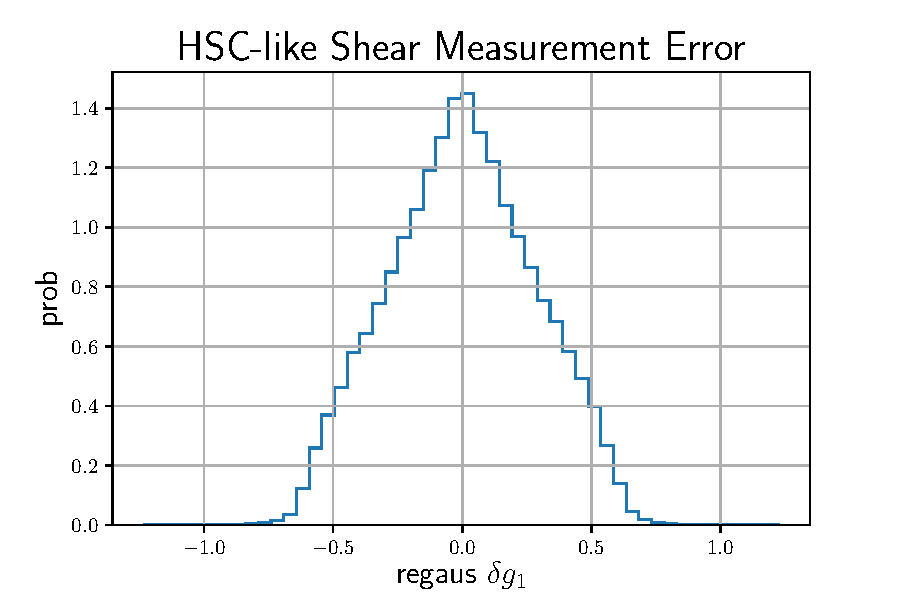
\includegraphics[width=0.45\textwidth]{shapeMeasurementError-HSCY1.pdf}
 \caption{The Histogram of HSC-like shear measurement error (including errors from shape noise and photon noise) on the 
        first component of shear ($g_1$).}
 \label{fig:mass-redshift}
\end{figure}

The observed galaxies have random irregular (unequally-spaced) spacial distribution. In order boost the computational
speed, we smooth the shear measurements from galaxy shapes and pixelize the smoothed measurements onto regular grids.
After the pixelization, the fast Fourier transform (FFT) can be directly conducted on the transverse plane in each 
source redshift bin.

The smoothing is conducted by convolving the shear measurements with a smoothing kernel
\begin{equation}
\gamma_{\rm{sm}} (\vec{\theta})  = \frac{\sum_i  W(\vec{\theta}-\vec{{\theta}}_i,z-z_i) \gamma_i}{\sum_i W(\vec{\theta}-\vec{{\theta}}_i,z-z_i) },
\end{equation}
where $W(\vec{\theta},z)$ is a $3$-D smoothing kernel. $\gamma_i$, $z_i$ and $\theta_i$ are the shear,
photometric reshift, and transverse position of the `$i$-th' galaxy in the catalog.

$W(\vec{\theta},z)$ can be decomposed into a transverse component $W_T(\vec{\theta})$ and a line-of-sight component
$W_\times(z)$
\begin{equation}
W(\vec{\theta},z)=W_T(\vec{\theta}) W_\times (z).
\end{equation}
In this paper, we use an isotropic $2$-D Gaussian kernel and a $1$-D top-hat kernel to smooth the measurements in the 
transverse plane and the line-of-sight direction, the smoothing kernel is 
\begin{equation}
\begin{split}
W_T(\vec{\theta}) &=\frac{1}{2\pi\beta^2}\exp(-\frac{|\vec{\theta}|}{2\beta^2}),\\
W_\times (z) &=
\begin{cases}
1/\Delta z& (|z|<\Delta z/2),\\
0& else.
\end{cases}
\end{split}
\end{equation}

With the approximation that the density of galaxy number ($n(\vec{r})$) varies slowly on the smoothing scale, 
since $\int d^3r W(\vec{r})=1$, the smoothed galaxy number density which is defined as
$$n_{\rm{sm}}(\vec{r})=\sum_i W(\vec{\theta}-\vec{\theta_i},z-z_i),$$
equals the number density. Therefore, we have $n_{\rm{sm}}(\vec{r})=n(\vec{r})$.
We note that the smooth approximation of the galaxy density does not hold near the boundary of the survey as
the galaxy number drop to zero outside of the boundary.

The smoothing operator is defined as
\begin{equation}
\mathbf{W} = \int d^3 r' W(\vec{r}-\vec{r'}),
\end{equation}
and the smoothing procedure influence the shear signal through
\begin{equation}
\gamma_L \rightarrow \mathbf{W} \gamma_L.
\end{equation}

As we will discussed in Section \ref{subsec:method-pixel}, the smoothed shear field is pixelized into an equally spaced
grids. Another widely used scheme is to directly average the shear measurements located in each pixel. Such scheme is 
equivalent to an equal-space sampling of the shear field smoothed with a $3$-D top-hat kernel with the same scale as 
the pixels.


\begin{figure}[!t]
 \centering
 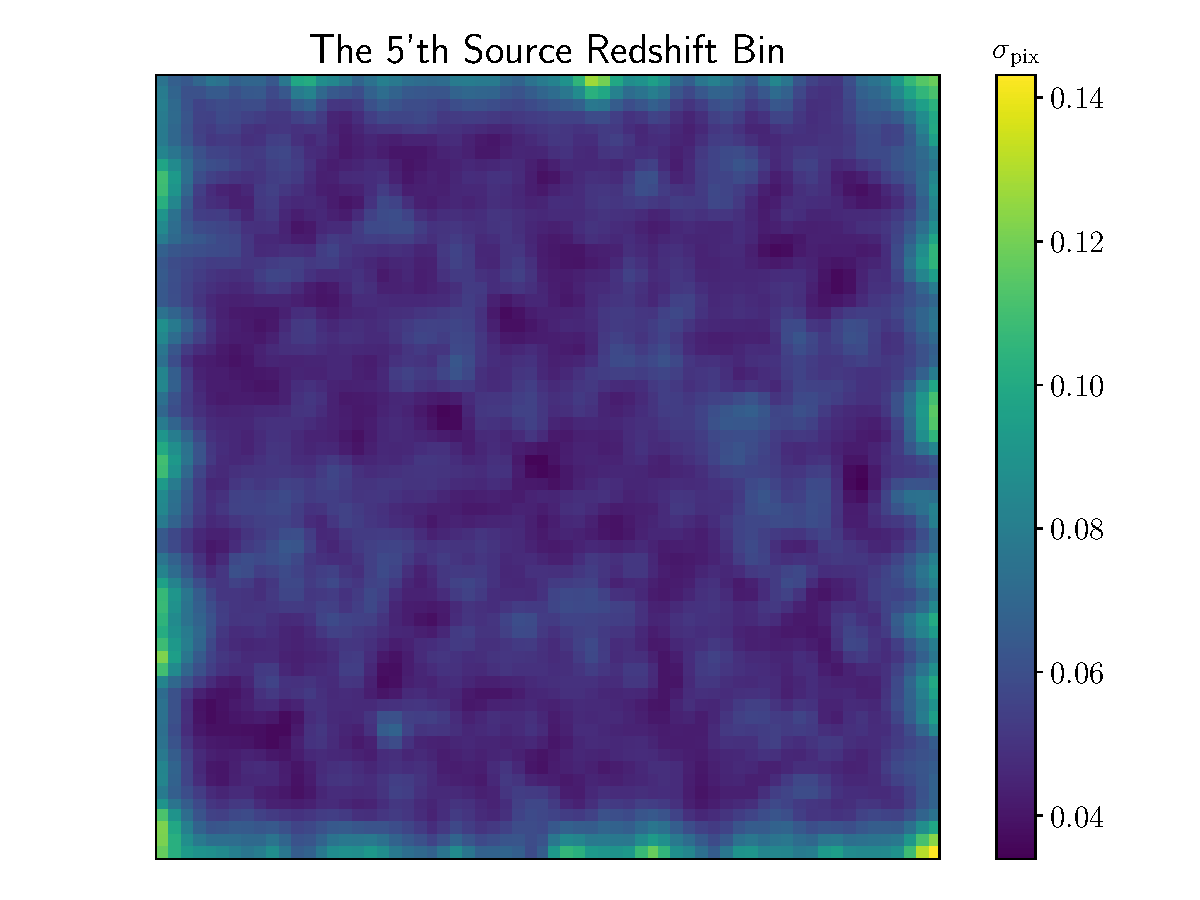
\includegraphics[width=0.45\textwidth]{noise_std_map_pix.pdf}
 \caption{The standard deviation map of shear measurement error for the fifth source bin ($0.69 \leq z < 0.80 $).}
\end{figure}

\subsubsection{Masking}
\label{subsec:method-msknoise}

\begin{figure*}[!t]
 \centering
 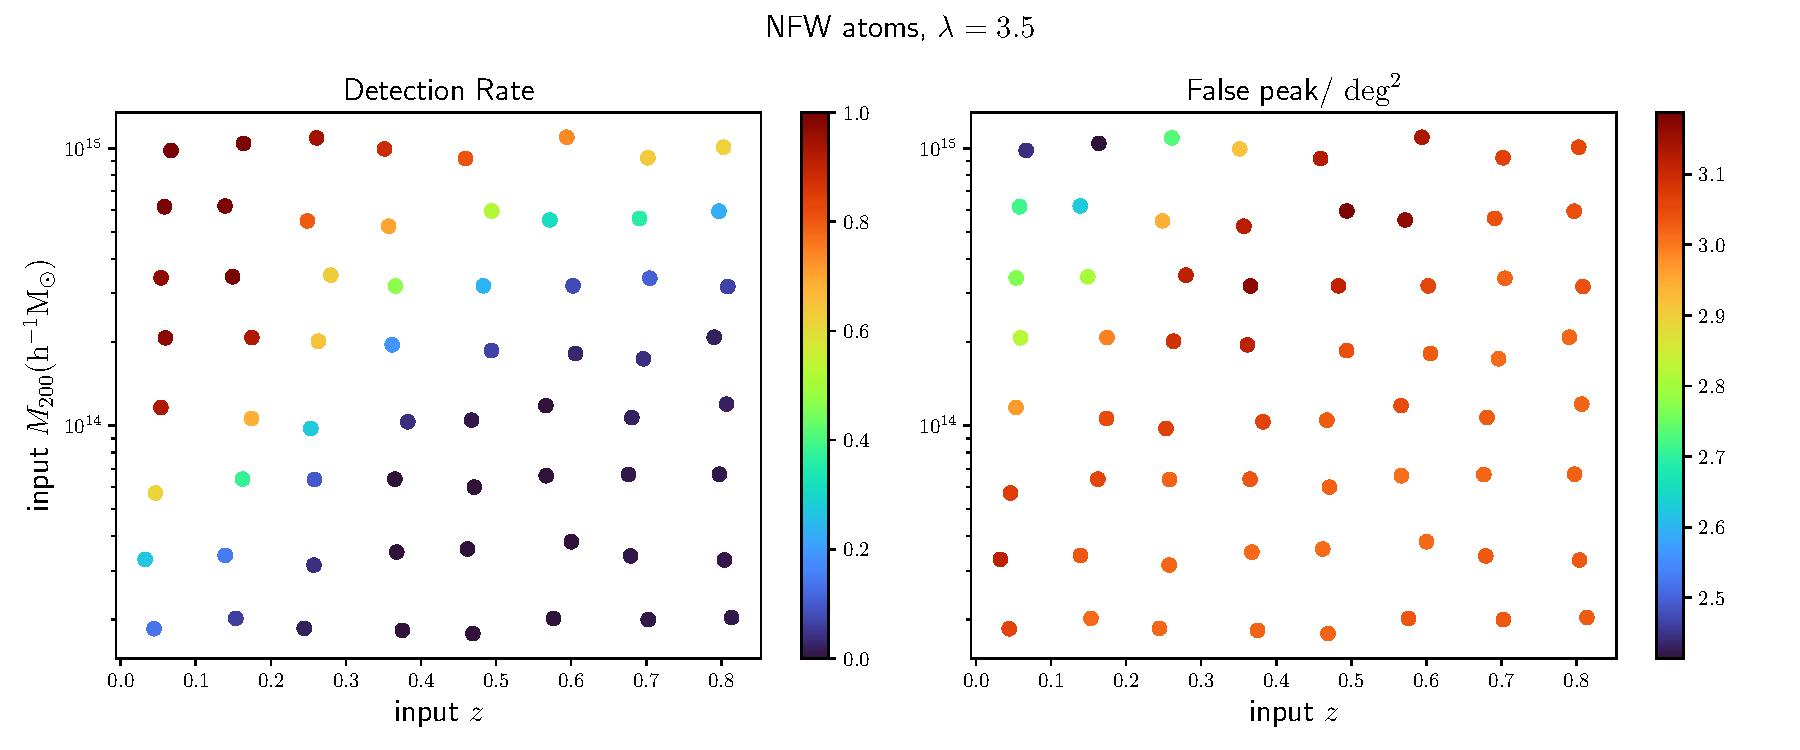
\includegraphics[width=0.95\textwidth]{detfalseRate_f3-1.pdf}
 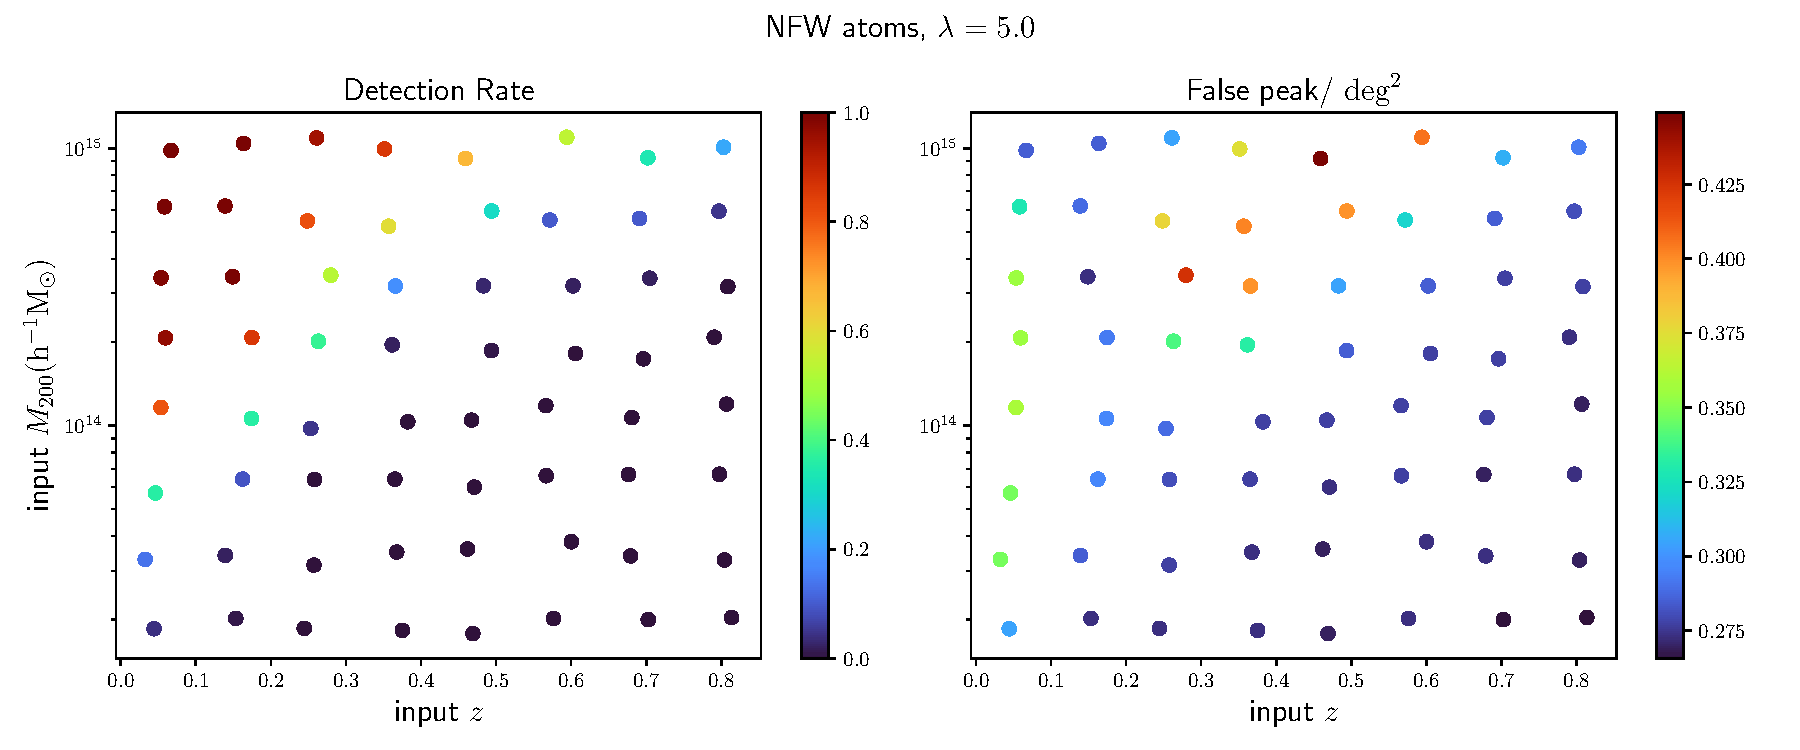
\includegraphics[width=0.95\textwidth]{detfalseRate_f3-3.pdf}
 \caption{The upper panels show the detection rate and false peak per square degree for mass map reconstruction with
NFW atoms and $\lambda=3.5$. The low panels show the results for $\lambda=5.0$. }
\end{figure*}

In real observations, shear measurements are available in a finite region of the sky and the boundary of the region is
always irregular. Moreover, there are also many isolated sub-regions do not have shear measurements due to the existence 
of neighboring bright stars or bad pixels.

We define the masking window function according to the smoothed number density of the galaxies as follows
\begin{equation}
 M(\vec{r})=
\begin{cases}
0 & n_{\rm{sm}}>1,\\
1 & \rm{else}.
\end{cases}
\end{equation}
The mask changes the shear measurements as
\begin{equation}\label{eq-delta2gamma-final}
\gamma_L(\vec{\theta},z) \rightarrow M(\vec{\theta},z) \gamma_L(\vec{\theta},z),
\end{equation}
We define the masking operator as
\begin{equation}
\mathbf{M}= \int d^3 r' M(\vec{r'}) \delta_D(\vec{r}-\vec{r'}),
\end{equation}
where $\delta_D(\vec{r})$ is $3$-D Dirac delta function. The shear is influenced by the masking through
$\gamma_L \rightarrow \mathbf{M} \gamma_L$.

The final observed shear field, taking into account all of the aforementioned systematics from observations,
is
\begin{equation}\label{eq-x2gamma-final}
\gamma =\mathbf{M} \mathbf{W} \mathbf{P} \mathbf{Q} \mathbf{\Phi} x.
\end{equation}
For simplicity, we denote $\mathbf{A}=\mathbf{M} \mathbf{W} \mathbf{P} \mathbf{Q} \mathbf{\Phi} $ and
eq. (\ref{eq-x2gamma-final}) is written as
\begin{equation}\label{eq-x2gamma-simple}
\gamma=\mathbf{A} x.
\end{equation}


\subsubsection{Pixelization}
\label{subsec:method-pixel}

\begin{figure*}[!t]
 \centering
 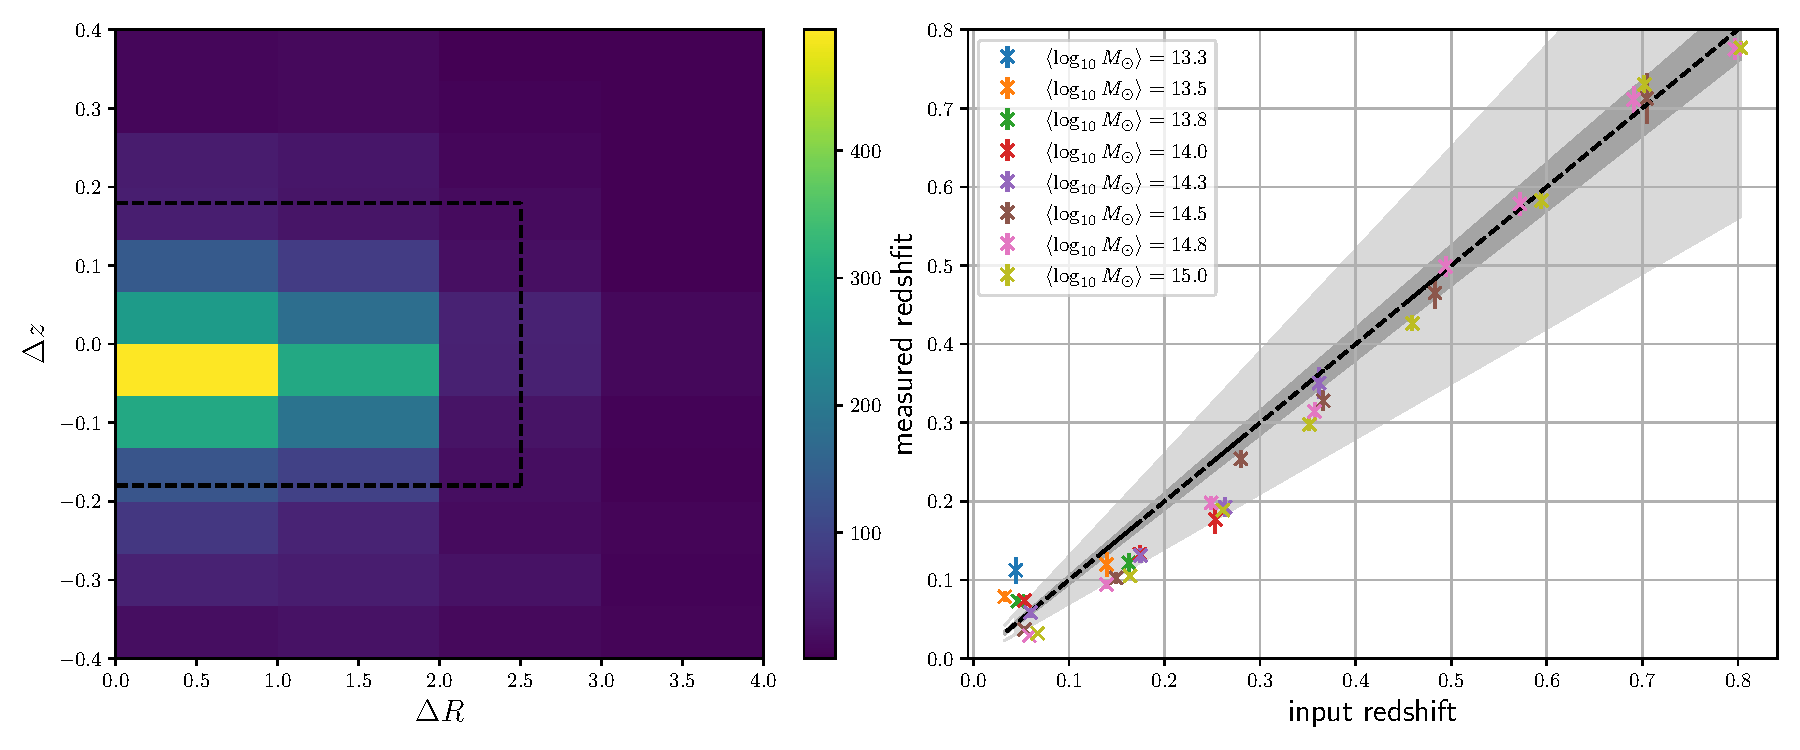
\includegraphics[width=0.95\textwidth]{peak_scatters_f3-1.pdf}
 \caption{The left panel shows the stacked distribution of deviations of detected peak positions 
 from the centers of the corresponding input halos. The $x$-axis is for the deviated distance in the transverse plane and the 
 $y$-axis is for the deviation of the redshift. The peaks inside the dashed black box are regarded as true detections. The 
 right panel focus on the deviation of detected peaks in the line-of-sight direction. The $x$-axis shows the input redshifts 
 and the $y$-axis is the redshift of the detected peak. The cross symbols show the average redshift of detected peak for 
 halos with different input redshift and mass and the error-bars are the scatter of the corresponding peak redshifts. All 
 of the results in this figure are based on the NFW atoms.}
\end{figure*}

We pixelize the smoothed shear field into a $N_\theta \times N_\theta \times N_s$ grid, where $N_\theta$
is the number of pixels of two orthogonal axes of the transverse plane and $N_s$ is the number of pixels of the
line-of-sight axis. $\gamma_{\alpha}$ is used to denote the value recorded on pixel with index $\alpha$, where $\alpha=
1...N_\theta \times N_\theta \times N_s$. The grids on the transverse plans are equally spaced, therefore fast Fourier
transform (FFT) can be used to boost the speed of linear operation on the transverse plan.

Similarly, we pixelize each scale frame of the parameter $x$ into a $N_\theta \times N_\theta \times N_l$ grid. 
The pixelization of the parameter field $x$ on the transverse plan for each scale frame is the same as the 
pixelization of the smoothed shear field on the transverse plane. $N_l$ is the number of the line-of-sight planes. 
$x_{\beta}$ is used to denote the element of the projected vector $x$ with index $\beta$, where $\beta=1...
N_\theta \times N_\theta \times N_l \times N$. The elements of the forward transform matrix $\mathbf{A}$ is denoted 
as $A_{\alpha\beta}$.

We term the column vectors of the transform matrix $\mathbf{A}$ as the effective basis atoms. We note that the effective 
basis atoms have different $l^2$ norm. The $l^2$ norm of the $i'th$ column vectors of the effective basis atoms are 
$\mathcal{N}_{i}=\sum_\alpha A_{i\alpha}A_{i\alpha}$. Before solving the density map reconstruction problem, we normalize 
the column
vectors of the transform matrix through the following rescaling
\begin{equation}
\begin{split}
A'_{\alpha\beta}&=A_{\alpha\beta}/\mathcal{N}_{\alpha}^{\frac{1}{2}},\\
x'_{\beta}&=x_{\beta}\mathcal{N}_{\beta}^{\frac{1}{2}}.\\
\end{split}
\end{equation}

\subsection{Density map reconstruction}
\label{subsec:method-reconstruction}

\subsubsection{Adaptive lasso}

The lasso algorithm uses $l^1$ penalty as the regularization term and the estimator is defined as
\begin{equation}
\hat{x'}^{\rm{lasso}}=\argmin_{x} \left\{ \frac{1}{2}\norm{\Sigma^{-\frac{1}{2}}(\gamma- \mathbf{A'} x')}_2^2+ \lambda_{\rm{ls}} \norm{x'}^1_1\right\},
\end{equation}
where $\norm{\bigcdot}_1$ and $\norm{\bigcdot}_2$ refer to the $l^1$ norm and $l^2$ norm, respectively. The $l^p$ norm is
defined as
\begin{equation}
\norm{x'}_p=(\sum_{i} |x'|^p_i)^{\frac{1}{p}},
\end{equation}
and $\lambda_{ls}$ is the penalization parameter for the preliminary lasso estimation.

Given that the parameters to measure is sparse, the lasso algorithm selects the parameters which are relevant to the 
measurements and simultaneously estimate the value of the selected parameters. However, it has been shown by 
\citet{AdaLASSO-Zou2006} that when the column vectors of the projection matrix $\mathbf{A'}$ are highly correlated, 
lasso cannot select the relevant parameters from the parameter space consistently. Moreover, the estimated parameters 
are biased due to the shrinkage process in the lasso regression. For the density map reconstruction problem, the effective
basis vectors are highly correlated since as shown in Figure \ref{fig-corlensKer}, the lensing kernels for lenses at 
different redshifts are highly correlated. Therefore, the lasso algorithm cannot select the consistent sparse model 
from the dictionary, which is demonstrated by the left figure of Figure \ref{fig-lassoVsadaLasso}.

\citet{AdaLASSO-Zou2006} proposes the adaptive lasso algorithm which uses adaptive weights to penalize different parameters
in the $l^1$ penalty. The addaptive lasso algorithm is a two-steps process. First, lasso is used to estimate the parameters and
the preliminary lasso estimation is denoted as $\hat{x'}^{\rm{lasso}}$. In the second step, the preliminary lasso estimation 
is used to weight the penalization. The weight on penalty is defined as
\begin{equation}
\hat{w}= \frac{1}{\abs{\hat{x'}^{\rm{lasso}}}^\tau},
\end{equation}
here we set the hyper-parameter $\tau$ to $2$. 
The adaptive lasso estimator is expressed as
\begin{equation}\label{eq-lossFun}
\hat{x'}=\argmin_{x'} \left\{ \frac{1}{2} \norm{\Sigma^{-\frac{1}{2}}(\gamma-\mathbf{A'}x')}^2_2 +
\hat{w}\lambda_{\rm{als}} \norm{x'}^1_1\right\}.
\end{equation}
Here $\lambda_{\rm{als}}$ is the penalization parameter for adaptive lasso which does not need to be the same as the 
penalization parameter for the preliminary lasso estimation ($\lambda_{\rm{ls}}$).

The loss function can be rewritten with Einstein notation
\begin{equation}
\begin{split}
L(x')&=\frac{1}{2}(\Sigma^{-1})_{\alpha\beta}(\gamma^{*}_{\alpha}-A'^{*}_{\alpha i}x'_{i})
(\gamma_{\beta}-A'_{\beta j}x'_{j})\\
&+ \lambda_{\rm{als}} \hat{w_\beta} \abs{x'_\beta}.
\end{split}
\end{equation}
To simplify the notification, we define the quadruple term in the loss function as $G(x')$:
\begin{equation}
G(x')=\frac{1}{2}\Sigma^{-1}_{\alpha\beta}(\gamma^{*}_{\alpha}-A'^{*}_{\alpha i}x'_{i})
(\gamma_{\beta}-A'_{\beta j}x'_{j}).
\end{equation}


\subsubsection{FISTA}

\begin{figure}[!t]
 \centering
 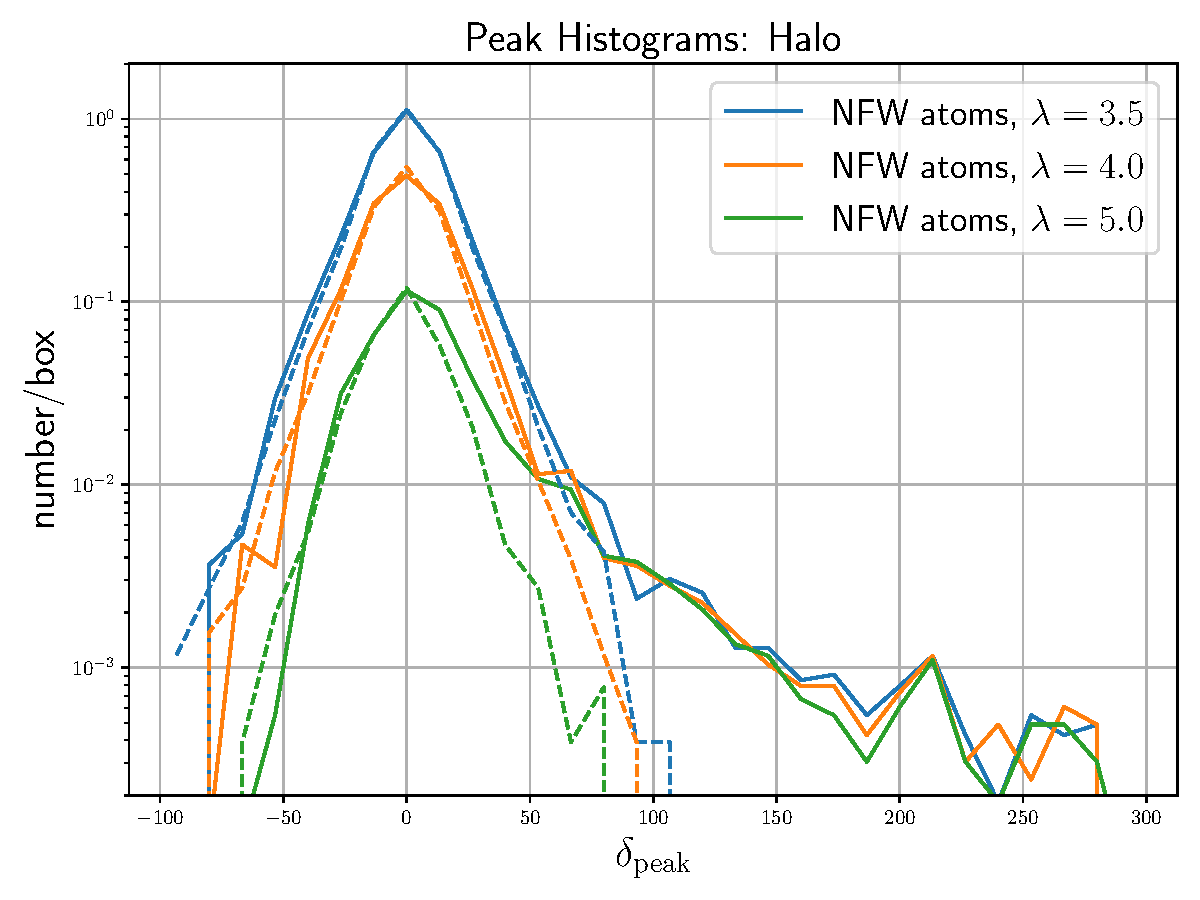
\includegraphics[width=0.45\textwidth]{peak_histograms.pdf}
 \caption{The histograms of detected peak values for all of the halo and error realizations. The dotted lines with different 
 colors are for the results of reconstruction with NFW atoms dictionary penalized with different regularization parameter 
 $\lambda$.}
\end{figure}

In this work, we apply the Fast Iterative Soft Thresholding Alorithm (FISTA) of \citet{FISTA-Beck2009} to solve 
the adaptive lasso estimator.

The parameters are initialized as $x_i^{(1)}=0$. According to the FISTA algorithm, we iteratively 
update the elements of the parameter vector ($x$). In the n'th iteration, a temporary update is first calcualted as
\begin{equation}
x'^{(n+1)}_{i}=\mathrm{ST}_{\lambda} \left(x'^{(n)}_{i} -\mu \partial_i G(x'^{(n)})\right),
\end{equation}
where $\mathrm{ST}$ is the soft thresholding function defined as
\begin{equation}
\mathrm{ST}_{\lambda} \left(x'\right) = \mathrm{sign} (x') \max \left(\abs{x'}-\lambda,0\right).
\end{equation}
$\mu$ is the step size of the gradient descent iteration. 
$\partial_i G(x'^{(n)})$ refers to the i'th element of the gradient
vector of $G$ at point $x'^{(n)}$
\begin{equation}
\partial_i G(x'^{(n)})=\Sigma^{-1}_{\alpha\beta}\Re\left(A'^{*}_{\alpha i}(\gamma_{\beta}-A'_{\beta j}x'_{j})\right),
\end{equation}
where $\Re\left( \bullet \right)$ is the function returns the real part of the input function.
The FISTA algorithm requires an additional step amounting to a weighted average between
$x'^{(n+1)}$ and $x'^{(n)}$:
\begin{equation}
\begin{split}
t^{(n+1)}&=\frac{1+\sqrt{1+4(t^{(n)})^2}}{2},\\
x'_{n+1} &\leftarrow x'^{(x+1)}+ \frac{t^{(n)}-1}{t^{(n+1)}}(x'^{(n+1)}-x'^{(n)}),
\end{split}
\end{equation}
where the relative weight is initialized as $t^{(1)}=1$.

Note that the FISTA algorithm coverges as long as the gradient descent step size $\mu$ satisfies
\begin{equation}
 0< \mu < \frac{1}{ \norm{\mathbf{A^{\dagger}} \mathbf{\Sigma}^{-1} \mathbf{A} }},
\end{equation}
where $\norm{\mathbf{A^{\dagger}} \mathbf{\Sigma}^{-1} \mathbf{A} }$ refers to the spectrum norm of the matrix
$\mathbf{A^{\dagger}} \mathbf{\Sigma}^{-1} \mathbf{A}$. The spectral norm is estimated using random
vectors. We simulate large number of random vectors with $l^2$ norms equal one with different realizations. Then, 
the matrix $\mathbf{A^{\dagger}} \mathbf{\Sigma}^{-1} \mathbf{A}$ is applied to each random vector and get a 
corresponding transformed random vector. The spectral norm of the matrix $\mathbf{A^{\dagger}} \mathbf{\Sigma}^{-1} \mathbf{A}$
is the maximum $l^2$ norm of the transformed vectors.


\subsubsection{The Algorithm}
The algorithm is described in Algorithm \ref{alg-1}.

\begin{algorithm}[H]
\renewcommand{\thealgorithm}{}
\label{alg-1}
\caption{Our Algorithm}
\begin{algorithmic}[1]
\INPUT $\gamma$: Pixelized complex $3$-D array of shear
\OUTPUT  $\delta$: $3$-D array of density contrast
\STATE Normalize column vectors of $\mathbf{A}$
\STATE Estimate step size $\mu$ and $\mathbf{\Sigma}$
\STATE \textbf{Initialization:} ‎
\STATE $x'^{(1)} = 0$ 
\STATE $\hat{w}=1$, $\lambda=\lambda_{\rm{ls}}$
\STATE $t^{(1)}=1$,$i=1$, $j=1$
\WHILE{$j \leq 2$}
    \WHILE{$i \leq N_{\rm{iter}}$}
        \STATE $x'^{(n+1)}_{i}=\mathrm{ST}_{\hat{w}\lambda} \left(x'^{(n)}_{i} -\mu \partial_i G(x'^{(n)})\right)$
        \STATE $t^{(n+1)}=\frac{1+\sqrt{1+4(t^{(n)})^2}}{2}$
        \STATE $x'_{n+1} \leftarrow x'^{(x+1)}+ \frac{t^{(n)}-1}{t^{(n+1)}}(x'^{(n+1)}-x'^{(n)})$
        \STATE $i=i+1$
    \ENDWHILE
\STATE \textbf{Reinitialization:} ‎
\STATE $\hat{w}=\abs{\hat{x'}^{\rm{lasso}}}^{-2}$, $\lambda=\lambda_{\rm{als}}$
\STATE $\hat{x'}^{(1)} = x'^{(N_{\rm{iter}})}$
\STATE $t^{(1)}=1$, $i=1$
\STATE $j=j+1$
\ENDWHILE
\STATE $\delta=\mathbf{\Phi}\mathcal{N}^{-\frac{1}{2}}x'^{(N_{\rm{iter}})}$
\end{algorithmic}
\end{algorithm}


\section{Tests}
\label{sec:Test}

\begin{figure*}[!ht]
 \centering
 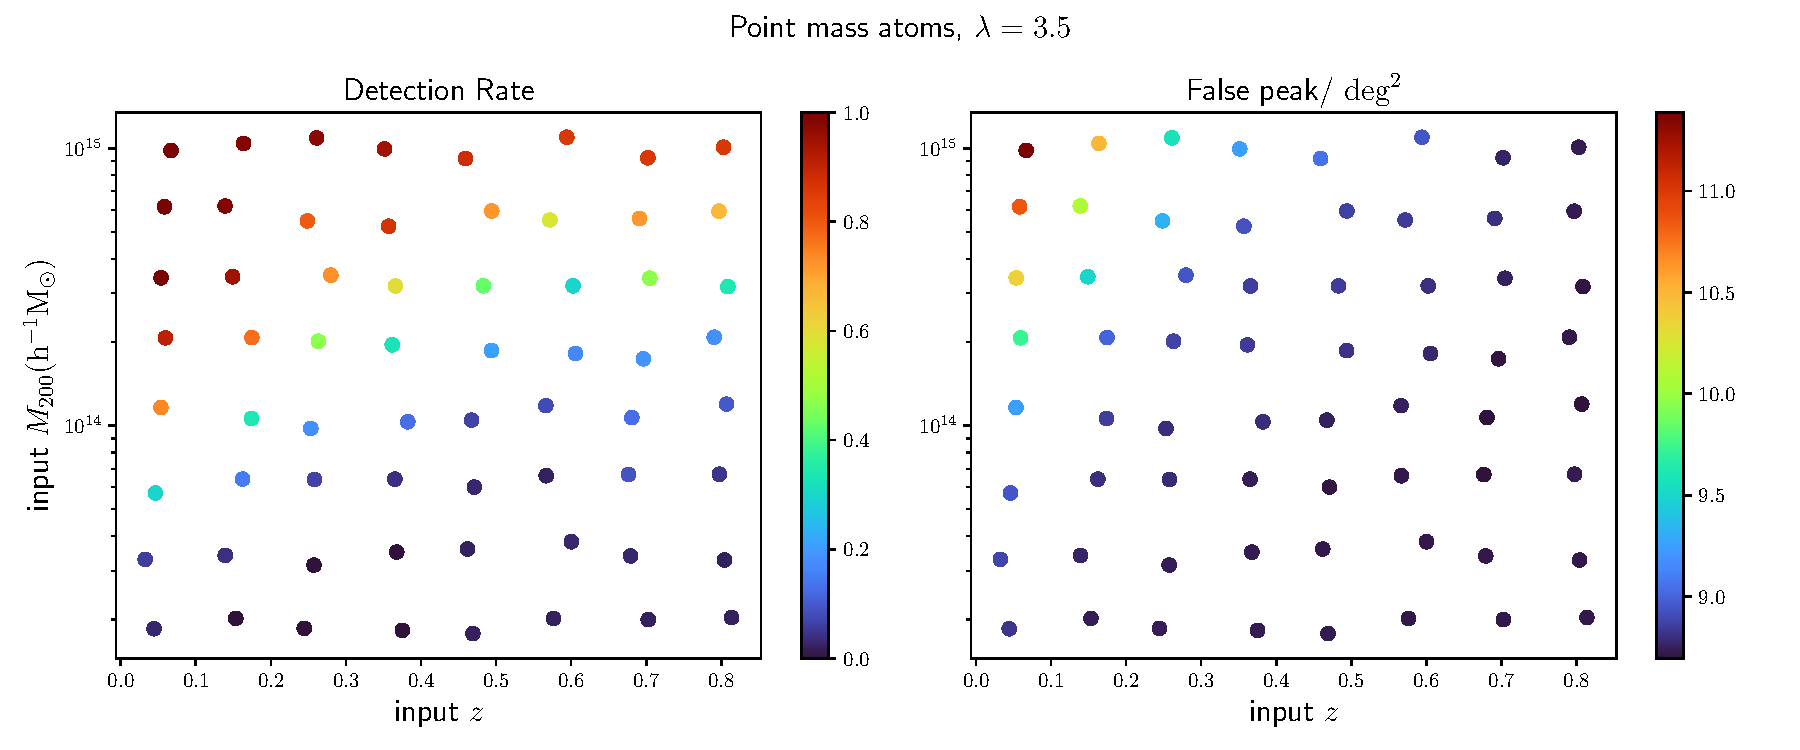
\includegraphics[width=0.95\textwidth]{detfalseRate_f1-1.pdf}
 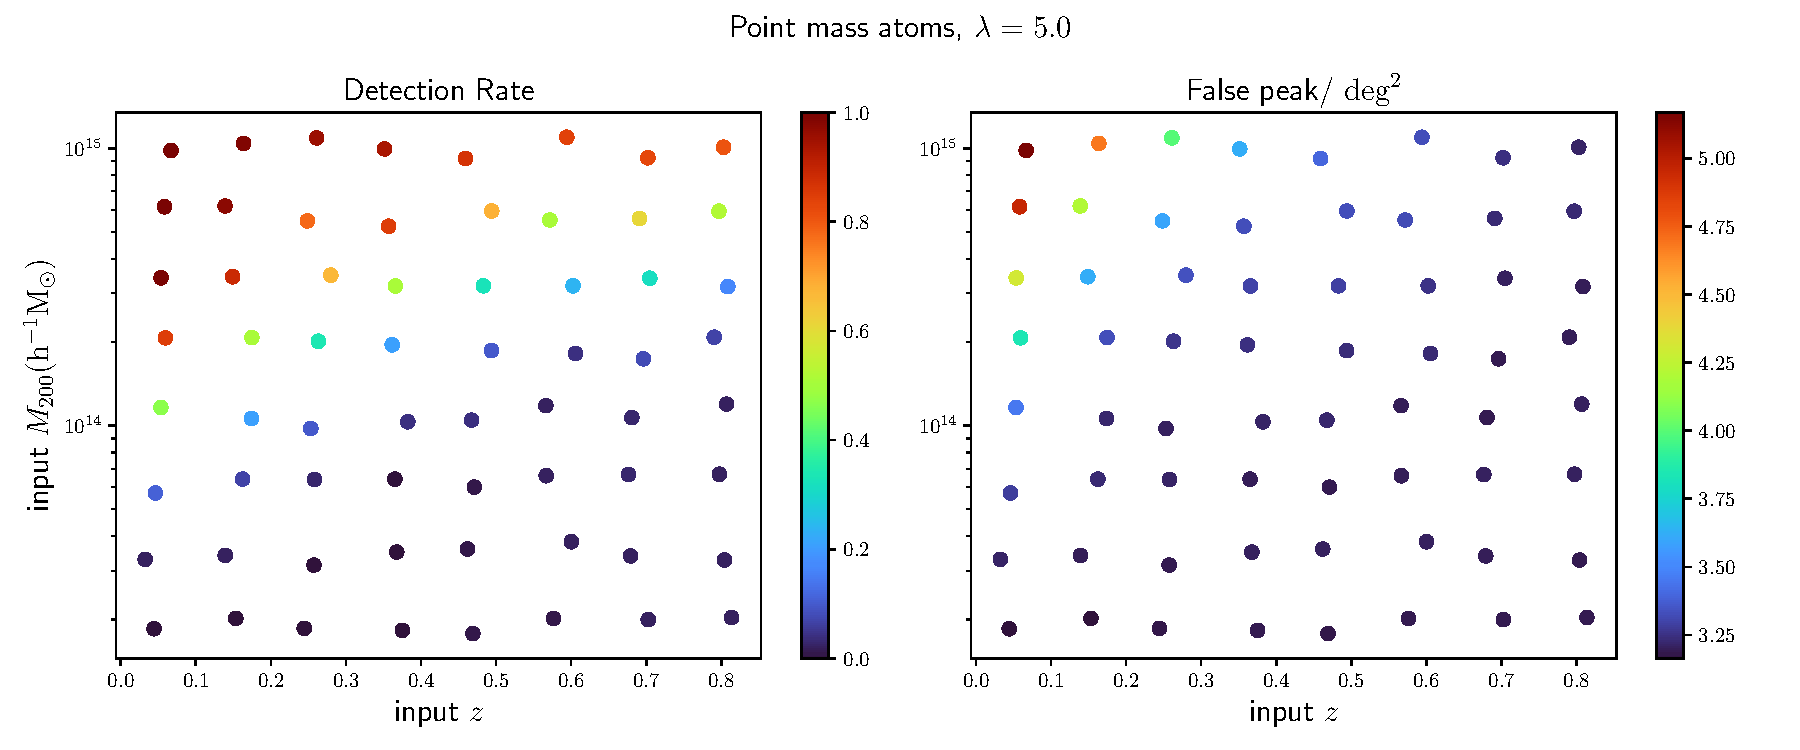
\includegraphics[width=0.95\textwidth]{detfalseRate_f1-3.pdf}
 \caption{The upper panels show the detection rate and false peak per square degree for mass map reconstruction with
point mass atoms and $\lambda=3.5$. The low panels show the results for $\lambda=5.0$. }
\end{figure*}

In this section, we simulate weak lensing shear fields induced by a group of halos with various halo masses 
and redshifts. The shear distortion fields are applied to HSC mock catalogs with different realizations of HSC-like shape 
noises and photo-$z$ uncertainties (Section \ref{subsec:Sims}).

Then, we test our algorithm on the simulations with two different setups of the algorithm. The first setup uses dictionary
constructed with NFW atoms (Section \ref{subsec:test-nfw}) and the second setup uses dictionary constructed with point mass 
atoms (Section \ref{subsec:test-pm}).

The $\Lambda$CDM cosmology used for the simulations is from the best fitting result of the final full-mission Planck observation 
of the cosmic microwave background (CMB) with $H_0=67.4 ~\rm{km~s^{-1} Mpc^{-1}}$ $\Omega_M=0.315$, $\Omega_\Lambda=0.685$
\citep{cmb-Planck2018-Cosmology}.

\subsection{Simulations}
\label{subsec:Sims}

We sample halos in two dimensional redshift-mass plane. The redshift-mass plane is evenly divided into eight redshift bins
and eight mass bins. The input redshifts and masses are shifted by random values for each halo from the centers 
of the bins.
The concentration of the NFW halo is a function of the halo's mass and redshift according to 
\citet{c-M_Magneticum-Ragagnin2019}
\begin{equation}
c_{h}=6.02\times(\frac{M_{200}}{10^{13} M_{\odot}})^{-0.12}(\frac{1.47}{1.+z_h})^{0.16}.
\end{equation}
The weak lensing shear fields of these NFW halos are simulated according to \citet{haloModel-TJ2003-3pt}. The shear 
distortions are applied to galaxy catalogs with HSC-like shape noise and photo-$z$ uncertainty. 

The galay catalogs are simulated with the HSC S16A shape catalog \citep{HSC1-catalog}. 
We uses galaxies in a one square degree region at the center of tract 9347 \citep{HSC1-data}.
By randomly rotating the galaxies in the shape catalog, we simulate HSC-like shear estimation errors 
with different realizations.
The positions of the galaxies are randomized so that the galaxies homogeneously distributed in a one square degree 
stamp.
For each galaxy, we randomly assign its redshift following the MLZ photo-$z$ probability distribution function 
\citep{HSC1-photoz} of the galaxy.

\subsection{NFW atoms}
\label{subsec:test-nfw}


\begin{figure*}[!t]
\centering
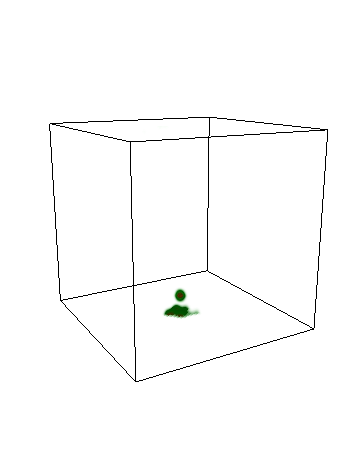
\includegraphics[width=0.42\textwidth]{delta-1-7-pz-wn-PM-falsepeakproblem.png}
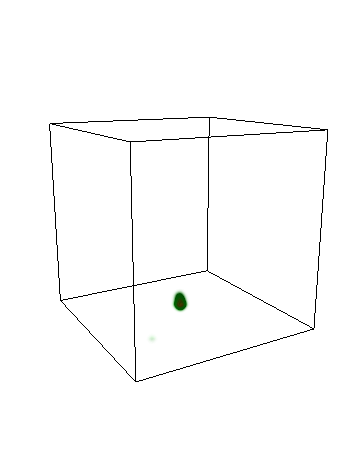
\includegraphics[width=0.42\textwidth]{delta-1-7-pz-wn-NFW-falsepeakproblem.png}
\caption{The result of density map reconstruction with  Point Mass atoms (left) and  NFW atoms (right). The input density 
        map is from a NFW halo with mass $M_{200}=10^{15.02} ~h^{-1}M_{\odot}$ at redshift $0.164$. The reconstruction 
        with point mass atoms has many false peaks at different redshfits.
        } \label{fig-lassoVsadaLasso}
\end{figure*}


In this subsection, we test the performance of our algorithm with the default setup which model the matter density
field with multi-scale NFW atoms. The dictionary space is constructed with NFW atom with NFW scale radius set to
three different comoving distances which are 0.12 Mpc/h, 0.24 Mpc/h, 0.36 Mpc/h. The truncation radius is set to
four times of the scale radius.
We test the algorithm with regularization parameter for the preliminary lasso is set to $3.5$ and $5.0$. The 
regularization parameter for the adaptive lasso is set to $\lambda_{\rm{als}}=\lambda_{\rm{ls}}^{\gamma+1}$.

\subsection{Point mass atoms}
\label{subsec:test-pm}
In this subsection, we test the performance of our algorithm with another setup which model the matter density
field with point mass atoms.
The dictionary space is constructed with point mass atoms in each lens redshift plane.
We also test the algorithm with regularization parameter for the preliminary lasso is set to $3.5$ and $5.0$. The 
regularization parameter for the adaptive lasso is set to $\lambda_{\rm{als}}=\lambda_{\rm{ls}}$.

Inspired by \citet{structureAdaLasso-Pramanik2020}, which propose to incorporate external group information into 
different penalization weights for the regression coefficients by setting the penalization weights for adaptive lasso
for model coefficients in the same group to the same value, we use a smoothed weight for adaptive lasso. The preliminary
lasso estimation is smoothed with a top-hat filter of comoving scale 0.25 Mpc/h, which is denoted as 
$\hat{x}^{\rm{ls}}_{\rm{sm}}$ and the penalization weights are set to $1/\abs{\hat{x}^{\rm{ls}}_{\rm{sm}}}^\gamma$.



\section{Summary}
\label{sec:Sum}

We develope a novel method to reconstruct $3$-D density contrast maps from photometric weak lensing shear measurements.
Our method models $3$-D density contrast maps as a summation of NFW atoms with multiple comoving radius and point mass atoms
in the $3$-D space binned with photometric redshift. The NFW atoms are used to model the mass in isolated halos and the 
point mass atoms are used to model the structures close to the resolution limit of the reconstruction. 

With the prior assumption that the basis atoms sparsely distributes in the $3$-D space, the density field is reconstructed 
using the adaptive lasso algorithm \citep{AdaLASSO-Zou2006} which has the oracle properties. 


The method is tested with realistic simulations using HSC-like shape noise and photo-$z$ uncertainties.


\bibliographystyle{aasjournal}
\bibliography{citation}

\appendix
\end{document}


\subsection{Pathwise Coordinate Descent Algorithm}
\label{subsec:method-pathwise}
\begin{figure}
 \centering
 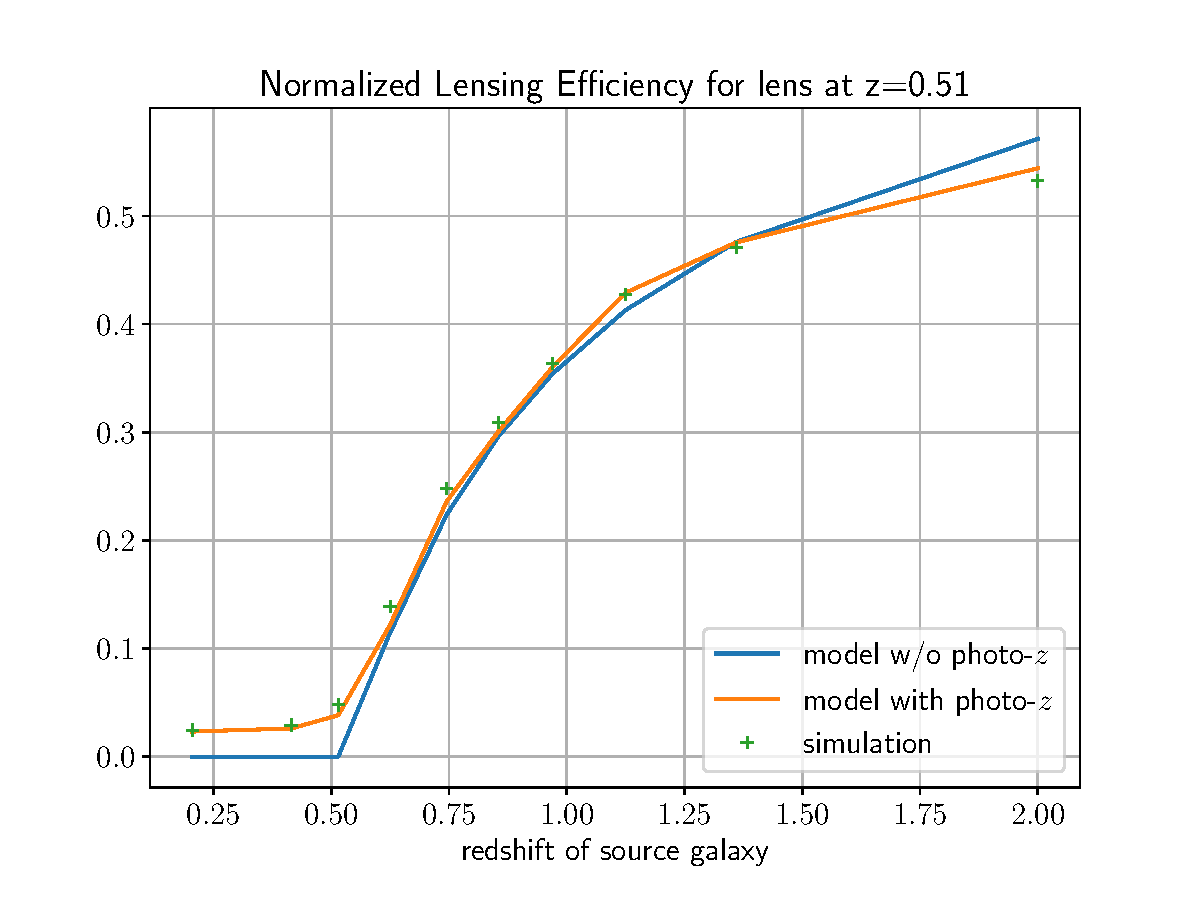
\includegraphics[width=0.5\textwidth]{lensing_efficiency.pdf}
 \caption{The blue line shows the normalized lensing efficiency for lens bin at $z_{l}=0.51$.
 The orange line is the normalized lensing efficiency while taking into account the photo-$z$ uncertainty.
 The green data points show the averaged $\kappa$ field for different redshift bins in the simulation.}
\end{figure}

The loss function can be separated into a summation of a quadratic term and a $l^1$ term as
\begin{equation}
 L(x)=G(x)+\lambda\sigma_{\beta}\norm{x_{\beta}}_1.
\end{equation}
The quadratic term is defined as
\begin{equation}
\begin{split}
 G(x)&=\frac{1}{2}(\gamma_{\alpha}-A^{*}_{\alpha\beta}x_{\beta})(\gamma_{\alpha}-A_{\alpha\mu}x_{\mu})\\
&+\frac{\tau}{2}[(D^{1}_{\alpha\beta} x_{\beta})(D^{1}_{\alpha\mu}x_{\mu})
+ (D^{2}_{\alpha\beta} x_{\beta})(D^{2}_{\alpha\mu}x_{\mu})],
\end{split}
\end{equation}

Many algorithms have been proposed to find the minima of this kind of loss function. We base our method on the
coordinate descent algorithm \citep{coordinateDescent-Wright2015} which is described as follows.
Firstly, we initialize the projector as $x^{(1)}=0$. According to the coordinate descent algorithm, we subsequently
update the projector ($x$) along the direction of one specific coordinate ($i$) as
\begin{equation}
x^{(n+1)}_{i}=\mathrm{ST}_{\lambda\sigma_{i}} (x^{(n)}_{i} -\frac{\partial_i G(x^{(n)})}{A_{\alpha i}A_{\alpha i}+4\tau}),
\end{equation}
where $\mathrm{ST}$ is the soft thresholding function defined as
\begin{equation}
\mathrm{ST}_{\lambda} (x) = \mathrm{sign} (x) \max (\abs{x}-\lambda,0),
\end{equation}
and the projector along the other coordinates are kept the same. The minima is finally approached by iteratively updating
along each coordinate for multiple times.

To simplify the notation, here we define the projector difference for the $n$-th iteration as
\begin{equation}
 \Delta x ^{(n)} = -\frac{\bigtriangledown G(x^{(n)})}{A_{\alpha i}A_{\alpha i}+4\tau},
\end{equation}
where $\bigtriangledown G(x^{(n)})$ refers to the gradient of quadratic function $G$ at $x^{(n)}$. The signal to noise ratio
(SNR) of the projector difference is defined as $s^{(n)}=\Delta x ^{(n)}/\sigma$.


In our algorithm, the coordinate descent algorithm in conducted in a pathwise manner \citep{pathwise-Friedman2007}.
We begin with a regulation parameter
($\lambda^{(1)}$) which is slightly smaller than the maximum coordinate of $s^{(1)}$ (denoted as $s_{\rm{max}}^{(1)}$) so that
in the first iteration, we only update on the coordinate with the maximum SNR. Then, we find the maximum projector difference
SNR of the second iteration ($s_{\rm{max}}^{(2)}$) and update the regulation parameter to $\lambda^{(2)}$, where $\lambda^{(2)}$
is slightly smaller than $s_{\rm{max}}^{(2)}$.

%$\mathrm{TSV}(x)$ refers to the total square variance of the first dictionary frame, which is defined as
%\begin{equation}
%\begin{split}
%\mathrm{TSV}(x) =\int d^2 \theta dz (\frac{\partial x}{\partial \theta_1})^2+\int d^2 \theta dz (\frac{\partial x}{\partial \theta_2})^2.
%\end{split}
%\end{equation}
%The total square variance can be expressed in a quadratic form as
%\begin{equation}
%\mathrm{TSV}(x)=\norm{\frac{\partial x}{\partial \theta_1}}^2_2+\norm{\frac{\partial x}{\partial \theta_2}}^2_2.
%\end{equation}
